\documentclass[10pt,a4paper]{article}
\usepackage[utf8]{inputenc}
\usepackage{amsmath}
\usepackage{amsfonts}
\usepackage{amssymb}
\usepackage{makeidx}
\usepackage{graphicx}
\usepackage{fullpage}

\usepackage{listings}
\usepackage{caption}
\usepackage{subcaption}
\captionsetup[lstlisting]{font=small}
\lstset{
	language=C,                % choose the language of the code
	numbers=left,                   % where to put the line-numbers
	stepnumber=1,                   % the step between two line-numbers.        
	numbersep=5pt,                  % how far the line-numbers are from the code
	showspaces=false,               % show spaces adding particular underscores
	showstringspaces=false,         % underline spaces within strings
	showtabs=false,                 % show tabs within strings adding particular underscores
	tabsize=2,                      % sets default tabsize to 2 spaces
	captionpos=b,                   % sets the caption-position to bottom
	breaklines=true,                % sets automatic line breaking
	breakatwhitespace=true,         % sets if automatic breaks should only happen at whitespace
}

\title{\centering 
	EED1005 Introduction to Programming	- Laboratory Quiz 2}
\begin{document}
	\maketitle	

		 1. a) Write flowchart for an algorithm that generate the sequence that elements of is determined as \indent  given rules.
		 b) Write c code of your flowchart (50p). 
		\begin{figure}[htbp]
			\centering
		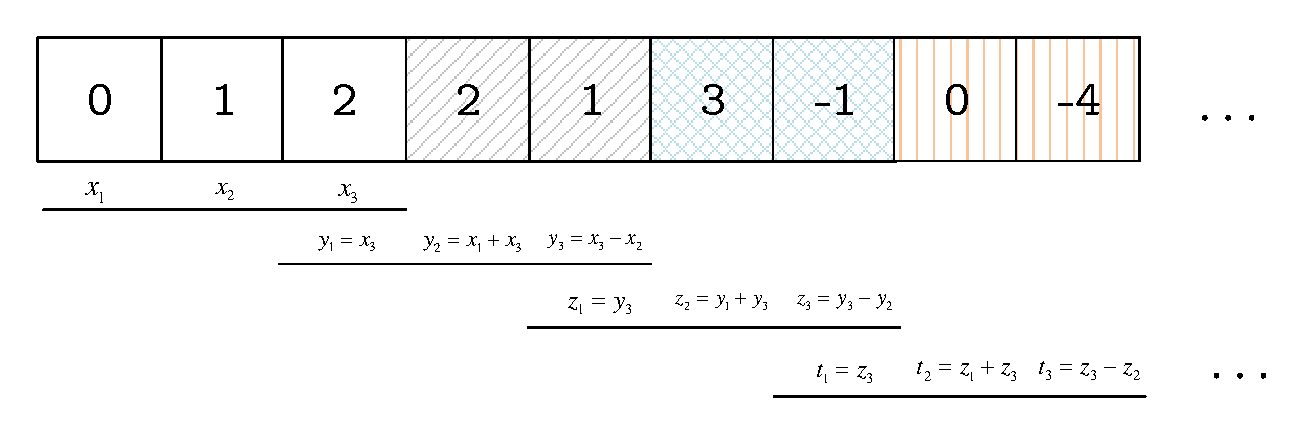
\includegraphics[scale=0.75]{sspdf}
		\end{figure}
		\begin{figure}[htbp]
		\centering
		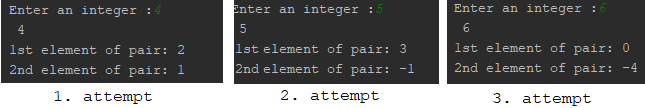
\includegraphics[scale=0.9]{ss2}
	\end{figure}
		
		\newpage
		

\end{document}